\documentclass[a4paper, 12pt]{article}
\usepackage[letterpaper]{geometry}
\geometry{top=0.2in, bottom=0.2in, left=0in, right=0in}

\usepackage{siunitx}
\usepackage{tikz}
\usepackage{pgfplots}
\usepackage{circuitikz}
\usepackage{caption}
\usepackage{amsmath}

\begin{document}

\pgfplotsset{
    every axis x label/.style={
        at={(ticklabel* cs:1.0)},
        anchor=west,
    },
    every axis y label/.style={
        at={(ticklabel* cs:0.9)},
        anchor=south east,
        align=center,
    },
    ylabel={$V_{out}/V_{in}$ \\ \si{\deci\bel}}, xlabel=$f$,
    axis x line = bottom, axis y line=left,
}

\quad \quad \quad {\huge \textbf{Filters}} \hline
\begin{figure}[h!] \caption*{\textbf{High pass RC filter (Differentiator)}}
    \centering
    \begin{minipage}{0.45\textwidth}
        \begin{circuitikz}[scale=0.8]
            \draw (0,0) to[C=C, o-] (2.5,0) to[short,-o] (5,0);
            \draw (2.5,0) to[resistor, R=R, *-*] (2.5,-3);
            \draw (0,-3) to[short, o-o] (5,-3); %negative pole
            \draw [|->] (0,-2.85) -- (0,-0.15) node[midway, fill=white]{$V_{in}$};
            \draw [|->] (5,-2.85) -- (5,-0.15) node[midway, fill=white]{$V_{out}$};
        \end{circuitikz}
    \end{minipage}
    \begin{minipage}{0.45\textwidth}
        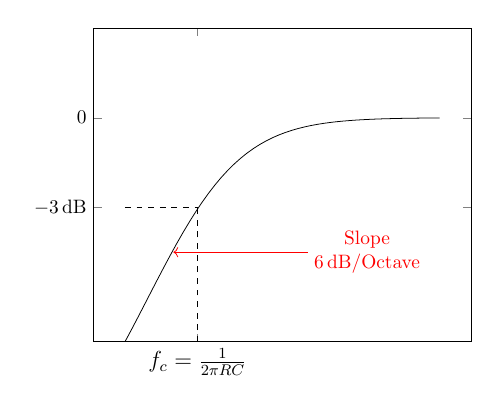
\begin{tikzpicture}[scale=0.7]
            \newcommand{\x}{0.3}
            \newcommand{\y}{0.3}
            \begin{axis}[
                ymin=0, ymax=0.7, domain = 0:1.3,
                xticklabel={\large $f_c = \frac{1}{2\pi RC}$}, yticklabels={\SI{-3}{\deci\bel}, 0},
                xtick={\x}, ytick={\y,0.5},
            ]
                \addplot[samples=50]{1/(1+ (x+1)^(-2*(2*x+2)) ) -0.5};
                \addplot[dashed] coordinates {(0,\y)(\x, \y)};
                \addplot[dashed] coordinates {(\x,0)(\x, \y)};
                \draw [->, red] (axis cs:1.0,0.2) node[fill=white, align=center] {Slope \\ \SI{6}{\deci\bel}/Octave} -- (axis cs:0.2,0.2);
            \end{axis}
        \end{tikzpicture}
    \end{minipage}
\end{figure}
\hline
\begin{figure}[h!] \caption*{\textbf{Low pass RC filter (Integrator)}}
    \centering
    \begin{minipage}{0.45\textwidth}
        \begin{circuitikz}[scale=0.8]
            \draw [|->] (0,-2.85) -- (0,-0.15) node[midway, fill=white]{$V_{in}$};
            \draw (0,0) to[resistor, R=R, o-] (2.5,0) to[short,-o] (5,0);
            \draw (2.5,0) to[C=C, *-*] (2.5,-3);
            \draw (0,-3) to[short, o-o] (5,-3); %negative pole
            \draw [|->] (5,-2.85) -- (5,-0.15) node[midway, fill=white]{$V_{out}$};
        \end{circuitikz}   
    \end{minipage}
    \begin{minipage}{0.45\textwidth}
        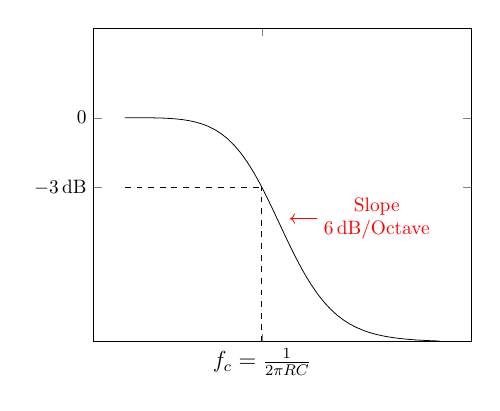
\begin{tikzpicture}[scale=0.7]
            \newcommand{\x}{0.87}
            \newcommand{\y}{0.69}
            \begin{axis}[
                ymin=0, ymax=1.4, domain = 0:2,
                xticklabel={\large $f_c = \frac{1}{2\pi RC}$}, yticklabels={\SI{-3}{\deci\bel}, 0},
                xtick={\x}, ytick={\y, 1},
            ]
            \addplot[samples=50]{1/(1+(x)^(2*(x+2)) )};
            \addplot[dashed] coordinates {(0,\y)(\x, \y)};
            \addplot[dashed] coordinates {(\x,0)(\x, \y)};
            \draw [->, red] (axis cs:1.6,0.55) node[fill=white, align=center] {Slope \\ \SI{6}{\deci\bel}/Octave} -- (axis cs:1.05,0.55);
            \end{axis}
        \end{tikzpicture}
    \end{minipage}
\end{figure}
\hline
\begin{figure}[h!] \caption*{\textbf{Band stop}}
    \centering
    \begin{minipage}{0.30\textwidth}
        \begin{circuitikz}[scale=0.8]
            \draw [|->] (0,-2.85) -- (0,-0.15) node[midway, fill=white]{$V_{in}$};
            \draw (0,0) to[resistor, R=R, o-] (2.5,0) to[short, -o] (5,0);
            \draw (2.5,0) to[inductor, L=L, *-] (2.5,-1.5) to[C=C, -*] (2.5,-3);
            \draw (0,-3) to[short, o-o] (5,-3); %negative
            \draw [|->] (5,-2.85) -- (5,-0.15) node[midway, fill=white]{$V_{out}$};
        \end{circuitikz}   
    \end{minipage}
    \begin{minipage}{0.30\textwidth}
        \begin{tikzpicture}[scale=0.7]
            \begin{axis}[
                ymin=-1.2, ymax=0, domain = -6:6,
                xticklabel={ \SI{-3}{\deci\bel} \\ B.W}, yticklabels={\SI{-40}{\deci\bel}, 0}, xticklabel style = {align=center},
                xtick={0}, ytick={-1.1, -0.3},
            ]
                \addplot[green!50!black] coordinates {(-1.2,-1.5)(-1.2,-0.5)};
                \addplot[green!50!black] coordinates {(1.2,-1.5)(1.2,-0.5)};
                \addplot[green!50!black, domain=-1.8:1.8] {-0.8};
                \addplot[samples=100] { (-1/(0.5*sqrt(2*pi))*exp(-((0.35*x-0)^2)/(2*0.4^2))) -0.3};
            \end{axis}
        \end{tikzpicture}
    \end{minipage}
    \begin{minipage}{0.30\textwidth}
        \begin{equation*}
            f_R = \frac{1}{2\pi \sqrt{LC}}
        \end{equation*}
    \end{minipage}
\end{figure}
\hline

\pagebreak
\begin{figure}[h!] \caption*{\textbf{Band Pass}}
    \centering
    \begin{minipage}{0.30\textwidth}
        \begin{circuitikz}[scale=0.8]
            \draw [|->] (0,-2.85) -- (0,-0.15) node[midway, fill=white]{$V_{in}$};
            \draw (0,0) to[resistor, R=R, o-] (2.5,0) to[short, -o] (5,0);
            \draw (2.5,0) to[short,*-*] (2.5,-0.5);
            \draw (2.5,-0.5) -- ++ (-0.5,0) to[inductor, a=L] ++(0,-2) -- ++ (1,0) to[capacitor, a=C] ++(0,2) -- ++ (-1,0); 
            \draw (2.5,-3) to[short,*-*] (2.5,-2.5);
            \draw (0,-3) to[short, o-o] (5,-3); %negative
            \draw [|->] (5,-2.85) -- (5,-0.15) node[midway, fill=white]{$V_{out}$};
        \end{circuitikz}   
    \end{minipage}
    \begin{minipage}{0.30\textwidth}
        \begin{tikzpicture}[scale=0.7]
            \begin{axis}[
                ymin=0, ymax=1.3, domain = -5:5,
                xticklabel={\large $f_R$}, yticklabels={0, \SI{40}{\deci\bel}},
                xtick={0}, ytick={0.1, 0.9},
            ]
                \addplot[green!50!black] coordinates {(-1.2,0)(-1.2,0.7)};
                \addplot[green!50!black] coordinates {(1.2,0)(1.2,0.7)};
                \addplot[green!50!black, domain=-1.8:2.5] {0.55};
                \addplot[samples=100] { 1/(0.5*sqrt(2*pi))*exp(-((0.35*x-0)^2)/(2*0.4^2)) + 0.1};
            \end{axis}
        \end{tikzpicture}
    \end{minipage}
    \begin{minipage}{0.30\textwidth}
        \begin{equation*}
            \begin{split}f_R = \frac{1}{2\pi \sqrt{LC}} \\
            Q = \frac{f_R}{\text{BW}}
            \end{split}
        \end{equation*}
    \end{minipage}
\end{figure}
\hline
\begin{figure}[h!] \caption*{\textbf{Twin T notch filter}}
    \centering
    \begin{minipage}{0.32\textwidth}
        \begin{circuitikz}[scale=0.8]
            \draw (0,0.5) to[short, o-*] (0.65,0.5) -- (0.65,1) -- (1.3,1) to[R=R] (3.3,   1) node[]{}
                to[R=R] (6.3,1) -- (6.3,0.5) to[short, *-o] (7,0.5);
            \draw (0.65,0.5) -- (0.65,0) to[capacitor,a=C] (3.3,0) to[capacitor,a=C] (6.3,0) -- (6.3,0.5);
            \draw (0,-3.5) to[short,o-o] (7,-3.5); %ground
            \draw (2.7,0) to[resistor, a=$\frac{R}{2}$, *-*] (2.7,-3.5);
            \draw (3.8,-3.5) node[circ]{} to[capacitor, a=2C] (3.8,-0.2) -- ++ (0,0) arc (-90:90:0.2) -- (3.8,1) node[circ]{};
            \draw [|->] (0,-3.35) -- (0,0.35) node[midway, left]{$V_{in}$};
            \draw [|->] (7,-3.35) -- (7,0.35) node[midway, left]{$V_{out}$};
        \end{circuitikz}
    \end{minipage}
    \begin{minipage}{0.32\textwidth}
        \begin{circuitikz}[scale=0.8]
            \draw [|->] (0,0.15) -- (0,3.85) node[midway, fill=white]{$V_{in}$};
            \draw (0,0) to[short, o-o] (7,0); %ground
            \draw (0,4) node[ocirc]{} -- (5.5,4) to[resistor, a=R] (5.5,1.5) to[capacitor, a=2C] (5.5,0) node[circ]{};
            \draw (1.5,0) node[circ]{} to[resistor, R=$\frac{R}{2}$] (1.5,1.5) to[capacitor, C=C] (1.5,4) node[circ]{};
            \draw (1.5,1.7) node[circ]{} to[capacitor,a=C] (3,1.7) to[resistor,R=R] (5.5,1.7) node[circ]{};
            \draw (3,1.7) node[circ]{} -- (3,3.85) -- ++ (0,0) arc(-90:90:0.15) -- (3,4.5) -- (7, 4.5) node[ocirc]{};
            \draw [|->] (7,0.15) -- (7,4.35) node[midway, fill=white]{$V_{out}$};
        \end{circuitikz}
        \caption*{Approx. \ang{67.5} phase shift in each "side" of bridge \& \ang{45} in "summing" RC pair}
    \end{minipage}
    \begin{minipage}{0.32\textwidth}
        \begin{tikzpicture}[scale=0.7]
            \begin{axis}[
                ymin=-1.2, ymax=0, domain = -6:6,
                xticklabel={{\Large $f_c = \frac{1}{2\pi RC} $}}, yticklabels={\SI{-40}{\deci\bel}, 0},
                xtick={0}, ytick={-1.1, -0.3},
            ]
                \addplot[samples=100] { (-1/(0.5*sqrt(2*pi))*exp(-((0.35*x-0)^2)/(2*0.4^2))) -0.3};
            \end{axis}
        \end{tikzpicture}
    \end{minipage}
\end{figure}

\end{document}
